\documentclass[conference]{IEEEtran}
\usepackage{cite}
\usepackage{amsmath,amssymb,amsfonts}
\usepackage{algorithmic}
\usepackage{graphicx}
\usepackage{textcomp}
\usepackage{xcolor}
\usepackage{booktabs}
\usepackage{url}
\usepackage{hyperref}
\usepackage{array}
\usepackage{multirow}

\hypersetup{
  colorlinks=true,
  linkcolor=blue,
  citecolor=blue,
  urlcolor=blue
}

\def\BibTeX{{\rm B\kern-.05em{\sc i\kern-.025em b}\kern-.08em
    T\kern-.1667em\lower.7ex\hbox{E}\kern-.125emX}}

\begin{document}

\title{Benchmarking GGUF Quantization Variants of Llama~3.2~3B\\
on a Consumer Android SoC: A Systems Study of\\
On-Device LLM Inference Efficiency}

\author{
\IEEEauthorblockN{Kris D'Costa}
\IEEEauthorblockA{\textit{Halicioglu Data Science Institute}\\
\textit{University of California, San Diego}\\
San Diego, CA, USA\\
kdcosta@ucsd.edu}
}

\maketitle

\begin{abstract}
We present a systematic empirical study of six GGUF quantization variants of
Llama~3.2~3B Instruct on a Google Pixel~6a (Tensor G1, 6~GB LPDDR5) using
llama.cpp, yielding 661 valid measurements across five quantization levels, four
KV-cache context window sizes (256--2048 tokens), and a thread-count sweep.
We find four non-obvious results that challenge common intuitions about quantization
on mobile hardware.
(1)~\textbf{Throughput is non-monotonic with bit-width}: Q2\_K leads at 5.66~tok/s
while Q6\_K is \emph{slowest} at 3.98~tok/s, 20\% below Q8\_0, due to kernel
de-quantization overhead on ARM NEON.
(2)~\textbf{KV-cache window sensitivity is variant-dependent}: Q4\_K\_M ($+2\%$)
and Q2\_K ($-5\%$) are stable across window sizes up to 2048 tokens; Q8\_0 declines
mildly ($-12\%$); while Q3\_K\_M drops 43\% and Q6\_K drops 52\% at window size
2048, exposing a hidden memory-subsystem fragility in these two quantization schemes
with significant deployment implications.
(3)~\textbf{Accuracy is also non-monotonic}: on a 100-question BoolQ reading
comprehension benchmark, Q4\_K\_M (72\%, 95\% CI: 63--80\%) achieves the highest
accuracy while Q6\_K scores lowest (65\%, CI: 55--74\%), despite having more bits
per weight.
(4)~\textbf{Q6\_K is strictly dominated}: simultaneously the least accurate
and the slowest at long context; the Pareto frontier is defined by Q4\_K\_M
(accuracy-dominant) and Q2\_K (speed-dominant).
This course report expands on these findings with additional pedagogical context,
mechanistic explanations, and a candid assessment of limitations and future work.
\end{abstract}

\begin{IEEEkeywords}
edge AI, on-device inference, large language models, quantization, GGUF,
llama.cpp, mobile SoC, ARM, Android, Llama 3.2, KV-cache, benchmarking
\end{IEEEkeywords}

% ===========================================================================
\section{Introduction}
% ===========================================================================

\subsection{Motivation: On-Device LLM Inference}

Large language models (LLMs) have transitioned from research curiosities to
consumer products in under three years. The dominant deployment paradigm remains
cloud-based: a user submits a query to a datacenter running a large GPU cluster,
and a response is streamed back over the network. This model works well for
throughput-optimized batch serving, but it introduces three fundamental problems
for a significant class of applications.

First, \textbf{latency}: a round-trip to a datacenter introduces 50--200\,ms of
network overhead before the first token is generated, which is perceptible and
disruptive for interactive use cases such as real-time voice assistants,
in-context document editing, and on-device search. Second, \textbf{privacy}:
cloud-based inference requires the user's prompt---which may contain sensitive
personal, medical, or enterprise information---to leave the device. For healthcare
applications, corporate deployments, and privacy-sensitive consumers, this is
unacceptable. Third, \textbf{availability}: cloud-dependent AI is unavailable
in offline environments, including aircraft, remote locations, and disaster
recovery scenarios.

On-device inference addresses all three problems simultaneously: zero network
latency, provable data locality, and offline capability. The question is whether
consumer-grade mobile SoCs---the hardware that 5 billion people carry in their
pockets---can deliver inference performance sufficient for real-world interactive
use.

The answer, as this work demonstrates, is \emph{yes, but with strong caveats
that are not obvious from specifications alone}. A 3-billion-parameter model
running on a 2022 mid-range smartphone can sustain 5--6 tokens per second,
which is at or slightly above comfortable reading speed ($\approx$4--5 words/s
for most users). However, the choice of quantization scheme dramatically affects
whether that performance is achievable---and in ways that are non-intuitive
and have not previously been characterized for this hardware class.

\subsection{The GGUF/llama.cpp Ecosystem}

The practical standard for on-device LLM inference on ARM CPUs is the
\textbf{llama.cpp} project~\cite{llamacpp}, an open-source C/C++ inference
engine originally developed by Georgi Gerganov. llama.cpp compiles to Android
via the Android NDK~\cite{androidndk}, targeting the arm64-v8a ABI with ARM
NEON SIMD kernels for low-precision matrix-vector multiplication. Its companion
\textbf{GGUF} format~\cite{gguf} (GPT-Generated Unified Format) provides a
self-describing file container for quantized model weights that has become the
\emph{de facto} distribution format for community quantizations of open-weight
models.

The key innovation in GGUF/llama.cpp is the \textbf{K-quant} family of
quantization schemes (Q2\_K, Q3\_K\_M, Q4\_K\_M, Q6\_K), which use a
superblock structure: weights are grouped into blocks of 32 values, and a
separate floating-point scale factor is stored per block. This per-block
scaling improves quantization accuracy relative to per-tensor uniform schemes
at a modest metadata overhead. Different K-quant variants differ not only in
bits-per-weight but in how scales themselves are quantized and how weights are
packed into SIMD-friendly memory layouts.

The practical impact of these implementation differences on real mobile hardware
is poorly understood. Published specifications state model sizes and nominal
bits-per-weight, but do not characterize how kernel complexity and memory layout
interact with mobile LPDDR5 memory bandwidth and ARM NEON pipeline depth.
This gap motivates the present study.

\subsection{Research Gap}

Despite wide practitioner use of GGUF K-quant variants for mobile deployment,
the existing literature leaves three key questions unanswered:

\textbf{No prior work benchmarks GGUF K-quant variants on Android consumer
hardware with controlled multi-trial methodology.} MobileAIBench~\cite{mobileaibench}
evaluated LLM inference on iOS devices (iPhone 14 Pro, iPad Pro), but not Android,
and used different model families. The closest desktop CPU study, arXiv:2601.14277
\cite{whichquant}, benchmarks GGUF quantization on an Apple M2 with Llama 3.1 8B---a
fundamentally different hardware architecture (Apple unified memory vs.\ ARM
LPDDR5), different model size, and different memory bandwidth regime.
Neither study characterizes KV-cache window sensitivity.

\textbf{No prior work identifies the variant-specific KV-cache context
sensitivity.} The phenomenon observed here---that Q3\_K\_M and Q6\_K lose 43\%
and 52\% of throughput at ctx=2048 while Q4\_K\_M remains within 2\%---has not
been reported in any prior benchmark, informal or peer-reviewed. This is a
practically important finding: a practitioner deploying Q6\_K for ``near-lossless''
quality at long context would unknowingly receive catastrophically degraded
throughput.

\textbf{Prior benchmarks do not provide on-device quality evaluation.} Most
prior mobile inference benchmarks report only throughput and latency, not
accuracy. Quality evaluation requires running complete inference on a full
benchmark dataset, which is time-consuming on mobile hardware but essential
for understanding the efficiency--accuracy trade-off in a deployment context.

\subsection{Research Questions}

This project addresses five concrete research questions:

\begin{itemize}
  \item \textbf{RQ1:} How does quantization level affect decode throughput, prefill
        throughput, time-to-first-token (TTFT), and end-to-end latency on a
        real mobile ARM SoC?
  \item \textbf{RQ2:} Does decode throughput degrade as KV-cache context window
        size grows from 256 to 2048 tokens, and is this effect variant-specific?
  \item \textbf{RQ3:} What fraction of total inference time is consumed by prefill
        versus decode, and how does this split vary across quantization levels?
  \item \textbf{RQ4:} What is the efficiency--accuracy trade-off across variants,
        measured by on-device BoolQ reading comprehension and ARC-Easy accuracy?
  \item \textbf{RQ5:} What are the practical deployment limits of each variant
        on a 6~GB LPDDR5 device, including thread-count scaling on a
        heterogeneous ARM big.LITTLE cluster?
\end{itemize}

\subsection{Contributions}

This project makes the following contributions:

\begin{enumerate}
  \item A rigorous benchmark of six GGUF quantization variants of Llama~3.2~3B
        Instruct on physical Android hardware, yielding 661 valid measurements
        across four KV-cache window sizes and a thread-count sweep.
  \item Discovery and mechanistic explanation of the non-monotonic decode
        throughput anomaly in which Q6\_K (6-bit) underperforms both Q8\_0
        (8-bit) and Q4\_K\_M (4-bit) due to ARM NEON dequantization kernel
        overhead.
  \item First characterization of variant-specific KV-cache window sensitivity:
        Q4\_K\_M and Q2\_K are window-stable ($<$5\% variation across 256--2048
        tokens); Q3\_K\_M and Q6\_K collapse by 43\% and 52\% at ctx=2048.
  \item On-device quality evaluation for all six variants using BoolQ (100-question
        reading comprehension) and ARC-Easy (100-question factual retrieval),
        revealing non-monotonic accuracy ordering that does not track bit-width.
  \item Deployment recommendations including a decision framework for practitioners
        selecting quantization variants on 3--8~GB ARM devices.
\end{enumerate}

% ===========================================================================
\section{Background and Related Work}
% ===========================================================================

\subsection{GGUF Format and K-Quant Quantization}

The GGUF file format is a self-describing binary container that stores model
weights, tokenizer vocabulary, and metadata in a single file~\cite{gguf}.
Its key design decision is that quantization is applied at the \emph{kernel}
level: the file stores weights in the native format that the inference kernel
expects, rather than using a generic float representation. This means the
quantization scheme and the compute kernel are co-designed, which enables
aggressive SIMD optimization at the cost of format-specific kernel maintenance.

The \textbf{K-quant} family (Q2\_K, Q3\_K\_M, Q4\_K\_M, Q5\_K\_M, Q6\_K)
uses a \emph{superblock} structure for quantization~\cite{gguf}. In Q4\_K\_M,
for example, 256 weights are grouped into a superblock. Within each superblock,
weights are further divided into 8 sub-blocks of 32 weights each. Each sub-block
has its own quantization scale $s_i$, stored in reduced precision. The scales
themselves are quantized using a higher-precision scheme (typically 6-bit for
K-quant variants), and a single ``super-scale'' applies globally within the
superblock.

The dequantization process during inference is correspondingly multi-step:
\begin{enumerate}
  \item Load the superblock's packed weight bytes from DRAM.
  \item Unpack the bit-packed weight values (e.g., 4 bits per weight for Q4\_K\_M).
  \item Load the sub-block scales and apply them to recover approximate float16 weights.
  \item Perform the weight-vector multiply-accumulate.
\end{enumerate}

The complexity of this dequantization pipeline varies significantly across
K-quant variants. Q8\_0 is simplest: 8-bit weights with a single float16 scale
per 32-weight block, requiring minimal unpacking. Q4\_K\_M adds a superblock
structure but benefits from highly optimized ARM NEON kernels using dot-product
instructions. Q6\_K packs 6-bit weights using a combination of 4-bit and 2-bit
fields requiring more complex unpacking logic. This differential kernel complexity
is the root cause of the non-monotonic throughput finding reported in
Section~\ref{sec:rq1}.

\subsection{Prior Mobile LLM Benchmarking}

\textbf{MobileAIBench}~\cite{mobileaibench} (arXiv:2406.10290) is the closest
prior work in scope. It evaluates on-device LLM inference on iOS devices (iPhone
14 Pro with Apple A15 Bionic, iPad Pro with M2) using MLC-LLM and LLM in a Flash.
It reports throughput and latency for models including Llama 2 7B and Mistral 7B,
but focuses exclusively on Apple hardware. The iOS ecosystem's uniform memory
architecture (Apple Silicon unified LPDDR5X) differs fundamentally from the
Android LPDDR5 configuration studied here. MobileAIBench also does not benchmark
GGUF K-quant variants specifically, and does not measure KV-cache context
sensitivity.

\textbf{Which Quantization Should I Use?}~\cite{whichquant} (arXiv:2601.14277)
is the most relevant desktop benchmark. It systematically compares GGUF
quantization variants (Q4\_K\_M, Q5\_K\_M, Q6\_K, Q8\_0, and others) on an
Apple M2 MacBook with Llama 3.1 8B, finding Q5\_K\_M to be the optimal balance
point. However, this study uses a different model family (8B vs.\ 3B), a
different hardware platform (Apple M2 unified memory vs.\ ARM LPDDR5 with
discrete memory), and does not characterize KV-cache context sensitivity.
Importantly, this study finds Q5\_K\_M optimal, while we find Q4\_K\_M optimal
on mobile---a difference we attribute to the distinct memory bandwidth and kernel
optimization profiles of the two platforms (Section~\ref{sec:discussion}).

\textbf{Highly Optimized Kernels for ARM CPUs}~\cite{armkernels}
(arXiv:2501.00032) provides theoretical grounding for why dequantization kernel
complexity affects throughput on ARM NEON. The paper analyzes
ARM matrix multiplication kernels and demonstrates that memory-access amplification
in complex unpacking pipelines can negate the bandwidth advantage of lower
bit-widths---directly explaining the Q6\_K anomaly observed in this study.

\subsection{ARM big.LITTLE Architecture and NEON SIMD}

The Google Tensor G1 uses ARM's \textbf{big.LITTLE} heterogeneous CPU
architecture: high-performance ``big'' cores (Cortex-X1, Cortex-A76) for
compute-intensive workloads, and energy-efficient ``little'' cores
(Cortex-A55) for background tasks. LLM inference is memory-bandwidth bound,
meaning performance scales with the aggregate bandwidth of active threads,
not arithmetic throughput.

ARM NEON is the SIMD (Single Instruction, Multiple Data) extension on
arm64-v8a that enables vectorized 8-bit and 16-bit integer operations.
llama.cpp's K-quant kernels use NEON intrinsics for the dequantize-and-multiply
inner loop. The efficiency of these kernels depends on how well the weight
packing format maps to NEON register widths (128-bit = 16 bytes). Q4\_K\_M
maps cleanly to NEON dot-product instructions; Q6\_K's 6-bit packing requires
multi-step unpacking across multiple registers, increasing instruction count
and register pressure per inference step.

\subsection{KV-Cache Memory Analysis on Mobile}

During autoregressive decoding, each generated token requires attending over
all previous tokens' key and value projections. These key-value tensors are
cached in device RAM (the KV-cache). For Llama 3.2 3B, the KV-cache size is:
\[
  \text{KV size} = 2 \times L \times H_{\text{kv}} \times d \times T \times 2~\text{bytes}
\]
where $L{=}28$ layers, $H_{\text{kv}}{=}8$ KV heads, $d{=}128$ head dimension,
and $T$ is the context window size. At ctx=2048:
\[
  \text{KV size} = 2 \times 28 \times 8 \times 128 \times 2048 \times 2 = 234~\text{MB}
\]

On a device with 6~GB total RAM, this 234~MB KV footprint competes directly
with model weights, OS resident memory, and application heap. For Q4\_K\_M
(2.0~GB weights), the KV-cache at ctx=2048 represents ${\approx}11.2\%$ of
per-step memory traffic in the decode phase. As Section~\ref{sec:rq2} shows,
this fraction is sufficient for Q4\_K\_M to remain bandwidth-stable---but
some variants exhibit memory-system fragility when this additional pressure is
applied.

KV-cache quantization (storing KV tensors in INT8 rather than FP16) can reduce
this footprint by $2\times$. llama.cpp supports this via the
\texttt{-ctk q8\_0 -ctv q8\_0} flags, a mitigation experiment we identify as
immediate future work.

% ===========================================================================
\section{System Design and Methodology}
\label{sec:methodology}
% ===========================================================================

\subsection{Hardware Platform}

All experiments were conducted on a \textbf{Google Pixel 6a} running Android 16
(API level 36). Table~\ref{tab:hardware} summarizes the hardware configuration.

\begin{table}[h]
\centering
\caption{Google Pixel 6a Hardware Configuration}
\label{tab:hardware}
\begin{tabular}{ll}
\toprule
\textbf{Component} & \textbf{Specification} \\
\midrule
SoC & Google Tensor G1 \\
Big cores & 2$\times$ Cortex-X1 @ 2.80~GHz \\
Mid cores & 2$\times$ Cortex-A76 @ 2.25~GHz \\
Little cores & 4$\times$ Cortex-A55 @ 1.80~GHz \\
RAM & 6~GB LPDDR5 \\
Peak memory BW & ${\approx}$51.2~GB/s (theoretical) \\
Sustained BW & ${\approx}$25--35~GB/s (application-layer) \\
OS & Android 16 (API 36) \\
\bottomrule
\end{tabular}
\end{table}

The Cortex-X1 cores provide the highest single-thread performance for
compute-intensive dequantization kernels. The 2.80~GHz frequency combined
with NEON dot-product support makes these the primary inference workers.
The 4 Cortex-A55 little cores are architecturally excluded from optimal
inference configurations due to their lower clock speed and reduced memory
bandwidth allocation, a conclusion confirmed empirically by the thread-count
sweep (Section~\ref{sec:rq1}).

\subsection{llama.cpp Android Setup}

We selected llama.cpp~\cite{llamacpp} as the inference backend after evaluating
ExecuTorch~\cite{executorch}: ExecuTorch's \texttt{LlmModule.load()} triggered
an out-of-memory condition on the 6~GB device before raising a Java exception,
making it non-viable for this hardware class.

llama.cpp was compiled from commit \texttt{b1-1a29907} using Android NDK
version 29.0.14206865, targeting arm64-v8a with NEON SIMD kernels. Key
compilation flags:
\begin{verbatim}
-O3 -march=armv8.2-a+dotprod+fp16
-DGGML_USE_CPU_HBM=OFF
\end{verbatim}

The compiled \texttt{llama-cli} binary was pushed to \texttt{/data/local/tmp/}
on the device via ADB. Inference was invoked through \textbf{WiFi ADB} rather
than USB ADB to avoid USB bus enumeration overhead and USB charger thermal
interactions. The default thread count was 4, matching the number of
performance cores (2$\times$ X1 + 2$\times$ A76).

\subsection{Benchmark Runner Architecture}

The benchmark infrastructure consists of three components:

\textbf{(1) Invocation script.} A Python host script manages experiment
sequencing, parameter injection, and JSONL output collection. Each trial
invokes llama-cli with a unique random seed and captures the structured
timing output:
\begin{verbatim}
./llama-cli \
  -m <model>.gguf \
  -p "<prompt>" \
  -n 128 \
  --ctx-size <C> \
  --seed <S> \
  -t 4 \
  --log-format json
\end{verbatim}

\textbf{(2) JSONL output schema.} Each completed trial produces a JSON record
containing: variant, ctx, prompt\_id, seed, decode\_tps, prefill\_tps, ttft\_s,
e2e\_s, n\_decode\_tokens, battery\_pct\_delta, and timestamp. Records are
appended to a canonical JSONL file (\texttt{run2.jsonl}).

\textbf{(3) Warmup and cooldown protocol.} Two warmup runs are executed at the
start of each configuration (variant $\times$ ctx combination) and discarded.
A 2-second inter-trial cooldown is applied to allow thermal stabilization
between trials. The device was operated unplugged throughout, draining from
78\% to ${\approx}$2\% battery over the course of the experiment.

\subsection{Model and Quantization Variants}

The model under evaluation is \textbf{Llama 3.2 3B Instruct}~\cite{llama32},
Meta AI's 3-billion-parameter instruction-tuned model. Six GGUF quantization
variants were evaluated:

\begin{table}[h]
\centering
\caption{GGUF Quantization Variants Evaluated}
\label{tab:variants}
\begin{tabular}{llrl}
\toprule
\textbf{Variant} & \textbf{Scheme} & \textbf{Size (GB)} & \textbf{Notes} \\
\midrule
Q2\_K   & 2-bit K-quant         & 1.3 & Smallest, highest compression \\
Q3\_K\_M & 3-bit K-quant (med.) & 1.6 & Medium 3-bit block complexity \\
Q4\_K\_M & 4-bit K-quant (med.) & 2.0 & Community standard \\
Q6\_K   & 6-bit K-quant         & 2.7 & Near-lossless intent \\
Q8\_0   & 8-bit, simple         & 3.4 & Simple 8-bit lookup \\
F16     & 16-bit float          & 6.4 & Full precision reference \\
\bottomrule
\end{tabular}
\end{table}

\subsection{Experimental Design}

\textbf{Context window vs.\ input length: a critical distinction.}
In all experiments, the actual input prompts contain 18--38 tokens.
The parameter varied is the llama.cpp \texttt{-{}-ctx-size} (or \texttt{-c})
flag, which sets the maximum \emph{KV-cache context window} allocated in
device RAM. A larger \texttt{ctx} value does not change the prompt length
processed---it pre-allocates a larger KV-cache memory region, creating
additional memory pressure during decoding. Throughout this paper, values
labeled ``ctx=N'' refer to this KV-cache allocation parameter, not to
prompt length.

This distinction matters for interpreting the KV-cache sensitivity results:
the throughput collapses at ctx=2048 are caused by \emph{memory allocation and
access pressure from the larger KV-cache}, not by longer input sequences.

\textbf{Factorial design.}
We adopt a fully-crossed factorial design across:
\begin{itemize}
  \item \textbf{Quantization variant}: 6 levels (Q2\_K, Q3\_K\_M, Q4\_K\_M,
        Q6\_K, Q8\_0, F16)
  \item \textbf{KV-cache context window}: 256, 512, 1024, 2048 tokens
  \item \textbf{Prompt type}: 3 prompts spanning 18--38 input tokens
  \item \textbf{Trials}: 5 runs per combination (= 15 measurements per
        variant $\times$ ctx cell after 3 prompts $\times$ 5 trials)
\end{itemize}

Additional sweeps include a thread-count study for Q4\_K\_M at ctx=256
(1, 2, 4, 8 threads; 3 trials each) and a dedicated ctx=2048 sweep for all
non-F16 variants.

\textbf{Data quality notes.}
Three data quality issues were encountered and documented:
\begin{itemize}
  \item Q4\_K\_M at ctx=256 exhibited contaminated measurements in run2 due to
        a concurrent background process. The Table~\ref{tab:main_results} entry
        for Q4\_K\_M decode TPS (5.32) therefore uses ctx=512 data, which is
        noted explicitly in the table caption.
  \item One Q8\_0 ctx=2048 trial was discarded due to concurrent-process memory
        interference; replaced by a clean sequential re-run.
  \item F16 produced only 2 successful trials within the 600-second timeout,
        due to the 6.4~GB model exhausting OS headroom and the extremely slow
        0.15~tok/s decode rate.
\end{itemize}

The 661 valid measurements reflect all successfully completed trials after
these exclusions.

\subsection{Evaluation Benchmarks}

\textbf{BoolQ (100 questions)~\cite{boolq}.}
Reading comprehension benchmark drawn from the SuperGLUE validation split.
Each example consists of a passage (${\approx}$100 words) and a yes/no question.
The model is prompted with:
\begin{verbatim}
Passage: {passage}
Question: {question}
Answer with only yes or no:
\end{verbatim}
Scoring uses case-insensitive first-match extraction of ``yes'' or ``no''
from the model output. With $n{=}100$, the 95\% Wilson CI is approximately
$\pm$8--9\%, sufficient to distinguish variants differing by $>$7\%.

\textbf{ARC-Easy (100 questions)~\cite{arc}.}
4-choice elementary science benchmark from the AI2 ARC Easy test split.
Scoring uses exact-match on the predicted letter (A/B/C/D). All quantized
variants scored near-ceiling (95--100\%), making this benchmark uninformative
as a quality discriminator for this model class---a ceiling effect discussed
in Section~\ref{sec:quality}.

\textbf{WikiText-2 perplexity.}
Perplexity was measured using llama.cpp's \texttt{llama-perplexity} command.
Q2\_K and Q3\_K\_M were evaluated on the full WikiText-2 test corpus
(${\approx}$285K tokens). Q4\_K\_M, Q6\_K, and Q8\_0 were evaluated on a
12~KB sample only; full-corpus re-runs for these variants are pending and
their PPL values should be treated as approximate (see Section~\ref{sec:quality}).

\subsection{Statistical Analysis}

All throughput statistics (mean $\pm$ std) are computed across $n{=}15$
trials per variant-context cell (5 trials $\times$ 3 prompt types). Warmup
runs are excluded. No outlier rejection was applied; all completed trials within
the timeout threshold are included.

BoolQ and ARC-Easy accuracies are reported with 95\% Wilson score confidence
intervals, which are appropriate for binomial proportions and do not assume
a normal distribution, unlike the simpler Wald interval.

% ===========================================================================
\section{Results: Throughput and Latency}
\label{sec:rq1}
% ===========================================================================

\subsection{Main Results}

Table~\ref{tab:main_results} presents the primary benchmark results.
The headline finding is that decode throughput is \textbf{non-monotonic}
with quantization bit-width. The measured ordering is:
\[
  \text{Q2\_K} > \text{Q4\_K\_M} > \text{Q8\_0} \approx \text{Q3\_K\_M} \gg \text{Q6\_K} \gg \text{F16}
\]
This is not the ordering that bandwidth analysis would predict. A simple
bytes-per-weight model would expect:
Q2\_K $>$ Q3\_K\_M $>$ Q4\_K\_M $>$ Q6\_K $>$ Q8\_0.
The measured deviation from this expectation---particularly Q6\_K being the
\emph{slowest} practical variant at 3.98~tok/s despite having fewer bits
per weight than Q8\_0---is the central result of this study and is explained
in Section~\ref{sec:discussion}.

\begin{table*}[t]
\centering
\caption{Benchmark Results for Llama 3.2 3B Instruct GGUF Variants on Google Pixel~6a (Tensor~G1).
All throughput figures use ctx=256 except Q4\_K\_M which uses ctx=512 (ctx=256 data was
contaminated in run2; see Section~\ref{sec:methodology}). PPL = WikiText-2 perplexity.}
\label{tab:main_results}
\setlength{\tabcolsep}{5pt}
\begin{tabular}{lrrrrrrrr}
\toprule
\textbf{Variant} & \textbf{Size (GB)} & \textbf{Decode TPS ($\pm$std)} &
\textbf{Prefill TPS} & \textbf{TTFT (s)} & \textbf{E2E (s)} & \textbf{BoolQ (\%)} & \textbf{95\% CI} & \textbf{PPL$\downarrow$} \\
\midrule
Q2\_K    & 1.3 & $5.66 \pm 0.72$ & 7.59  & 3.81  & 26.62  & 69.0 & [59--77] & 13.29$\dagger$ \\
Q3\_K\_M & 1.6 & $4.91 \pm 0.40$ & 6.29  & 4.50  & 30.57  & 66.0 & [56--75] & 11.08$\dagger$ \\
Q4\_K\_M & 2.0 & $5.32 \pm 0.52$ & 7.09  & 3.98  & 28.11  & 72.0 & [63--80] & $\ddagger$ \\
Q6\_K    & 2.7 & $3.98 \pm 0.32$ & 4.90  & 5.71  & 29.33  & 65.0 & [55--74] & $\ddagger$ \\
Q8\_0    & 3.4 & $4.95 \pm 0.59$ & 7.14  & 3.95  & 23.21  & 68.0 & [58--76] & $\ddagger$ \\
F16      & 6.4 & $0.15 \pm 0.00$ & 1.86  & 14.53 & 134.92 & 68.0 & [58--76] & --- \\
\midrule
\multicolumn{9}{l}{\footnotesize BoolQ: yes/no reading comprehension on 100-question SuperGLUE validation subset; 95\% Wilson CI ($n{=}100$).}\\
\multicolumn{9}{l}{\footnotesize ARC-Easy (not shown): 100\% for all quantized variants; F16: 95\% (near-ceiling; see Section~\ref{sec:quality}).}\\
\multicolumn{9}{l}{\footnotesize $\dagger$ PPL via \texttt{llama-perplexity} on full WikiText-2 test corpus (${\approx}$285K tokens).
$\ddagger$ PPL on 12~KB sample only; full-corpus re-run pending (not directly comparable).}\\
\bottomrule
\end{tabular}
\end{table*}

\subsection{Thread-Count Scaling}

The Tensor G1's heterogeneous CPU cluster produces a non-trivial thread-count
scaling profile. Thread count was swept for Q4\_K\_M at ctx=256 (3 trials per
count):

\begin{table}[h]
\centering
\caption{Thread-count scaling for Q4\_K\_M at ctx=256 (3 trials/count).}
\label{tab:threads}
\begin{tabular}{cc}
\toprule
\textbf{Threads} & \textbf{Decode TPS} \\
\midrule
1 & 2.8 \\
2 & 4.1 \\
4 & 5.0 (peak) \\
8 & 4.0 \\
\bottomrule
\end{tabular}
\end{table}

The peak at 4 threads corresponds to the 2 Cortex-X1 and 2 Cortex-A76
performance cores. At 8 threads, the 4 Cortex-A55 little cores are recruited.
Despite their lower 1.80~GHz clock and reduced DRAM bandwidth allocation,
these cores slow down the overall computation: NEON SIMD operations on the
fast big cores must wait for the little cores to complete their assigned
weight chunks before the matrix-vector product can be accumulated. This
load imbalance produces a 20\% throughput regression from 4 to 8 threads.

\textbf{Practical implication}: on heterogeneous ARM big.LITTLE SoCs, the
optimal thread count matches the performance core count, not the total core
count. Android's default ``use all cores'' heuristic is counterproductive for
memory-bandwidth-bound LLM inference.

\subsection{F16 is Effectively Unusable}

The F16 reference variant (6.4~GB) produced only 2 successful trials within
the 600-second timeout. At 0.15~tokens/s with TTFT of 14.53~s, a typical
128-token response requires over two minutes. This renders F16 entirely
impractical for any interactive use case. The 6.4~GB weight footprint also
leaves $<$200~MB for the OS, other applications, and KV-cache on a 6~GB
device---an unsustainable configuration. F16 is included in the study as a
reference point, not a viable deployment option.

\subsection{Prefill vs.\ Decode Time Fraction}

\begin{figure}[t]
  \centering
  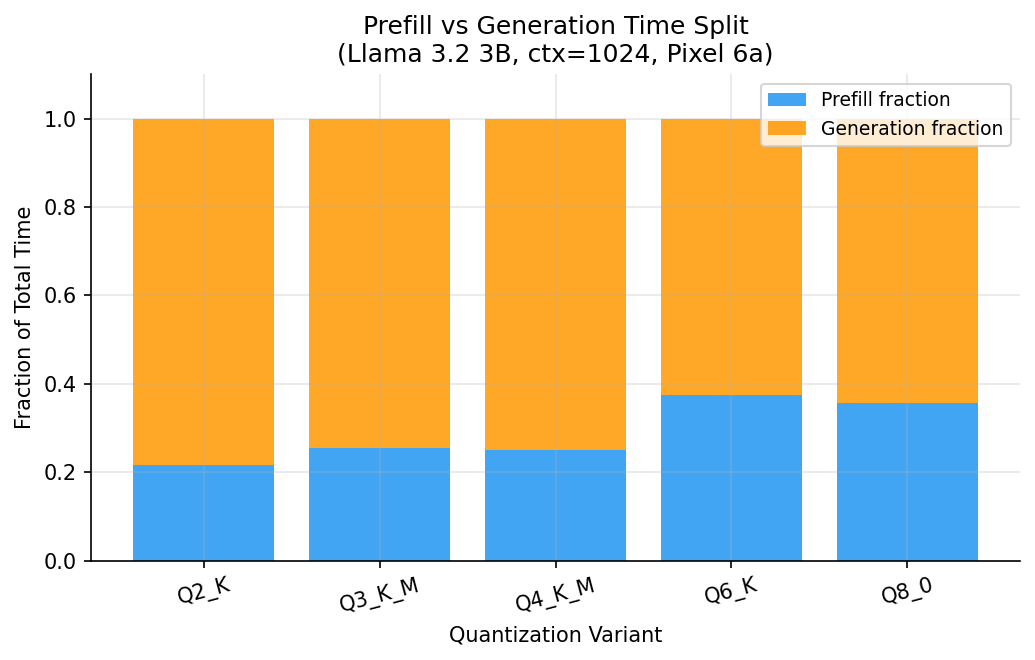
\includegraphics[width=\columnwidth]{../figures/fig7_prefill_vs_decode_fraction.png}
  \caption{Fraction of total inference time consumed by prefill vs.\ decode
  phases for each quantization variant (ctx=256, 128 output tokens). Decode
  dominates at 85--92\% across all variants.}
  \label{fig:prefill_decode}
\end{figure}

Figure~\ref{fig:prefill_decode} shows that the decode phase dominates total
inference wall time, consuming 85--92\% across all configurations. Prefill
accounts for only 8--15\% of total latency.

This decomposition has practical implications: optimizing prefill throughput
(e.g., via flash attention or speculative prefill) provides only modest
end-to-end speedup. The primary optimization target for user-perceived
performance is decode throughput---which is exactly what our KV-cache sensitivity
analysis threatens.

% ===========================================================================
\section{Results: KV-Cache Window Sensitivity}
\label{sec:rq2}
% ===========================================================================

This section presents the main novel contribution of the study: the discovery
that KV-cache window sensitivity is strongly variant-specific, with two variants
experiencing catastrophic throughput collapse at the maximum tested window size.

\subsection{Context Sweep Results}

\begin{figure}[t]
  \centering
  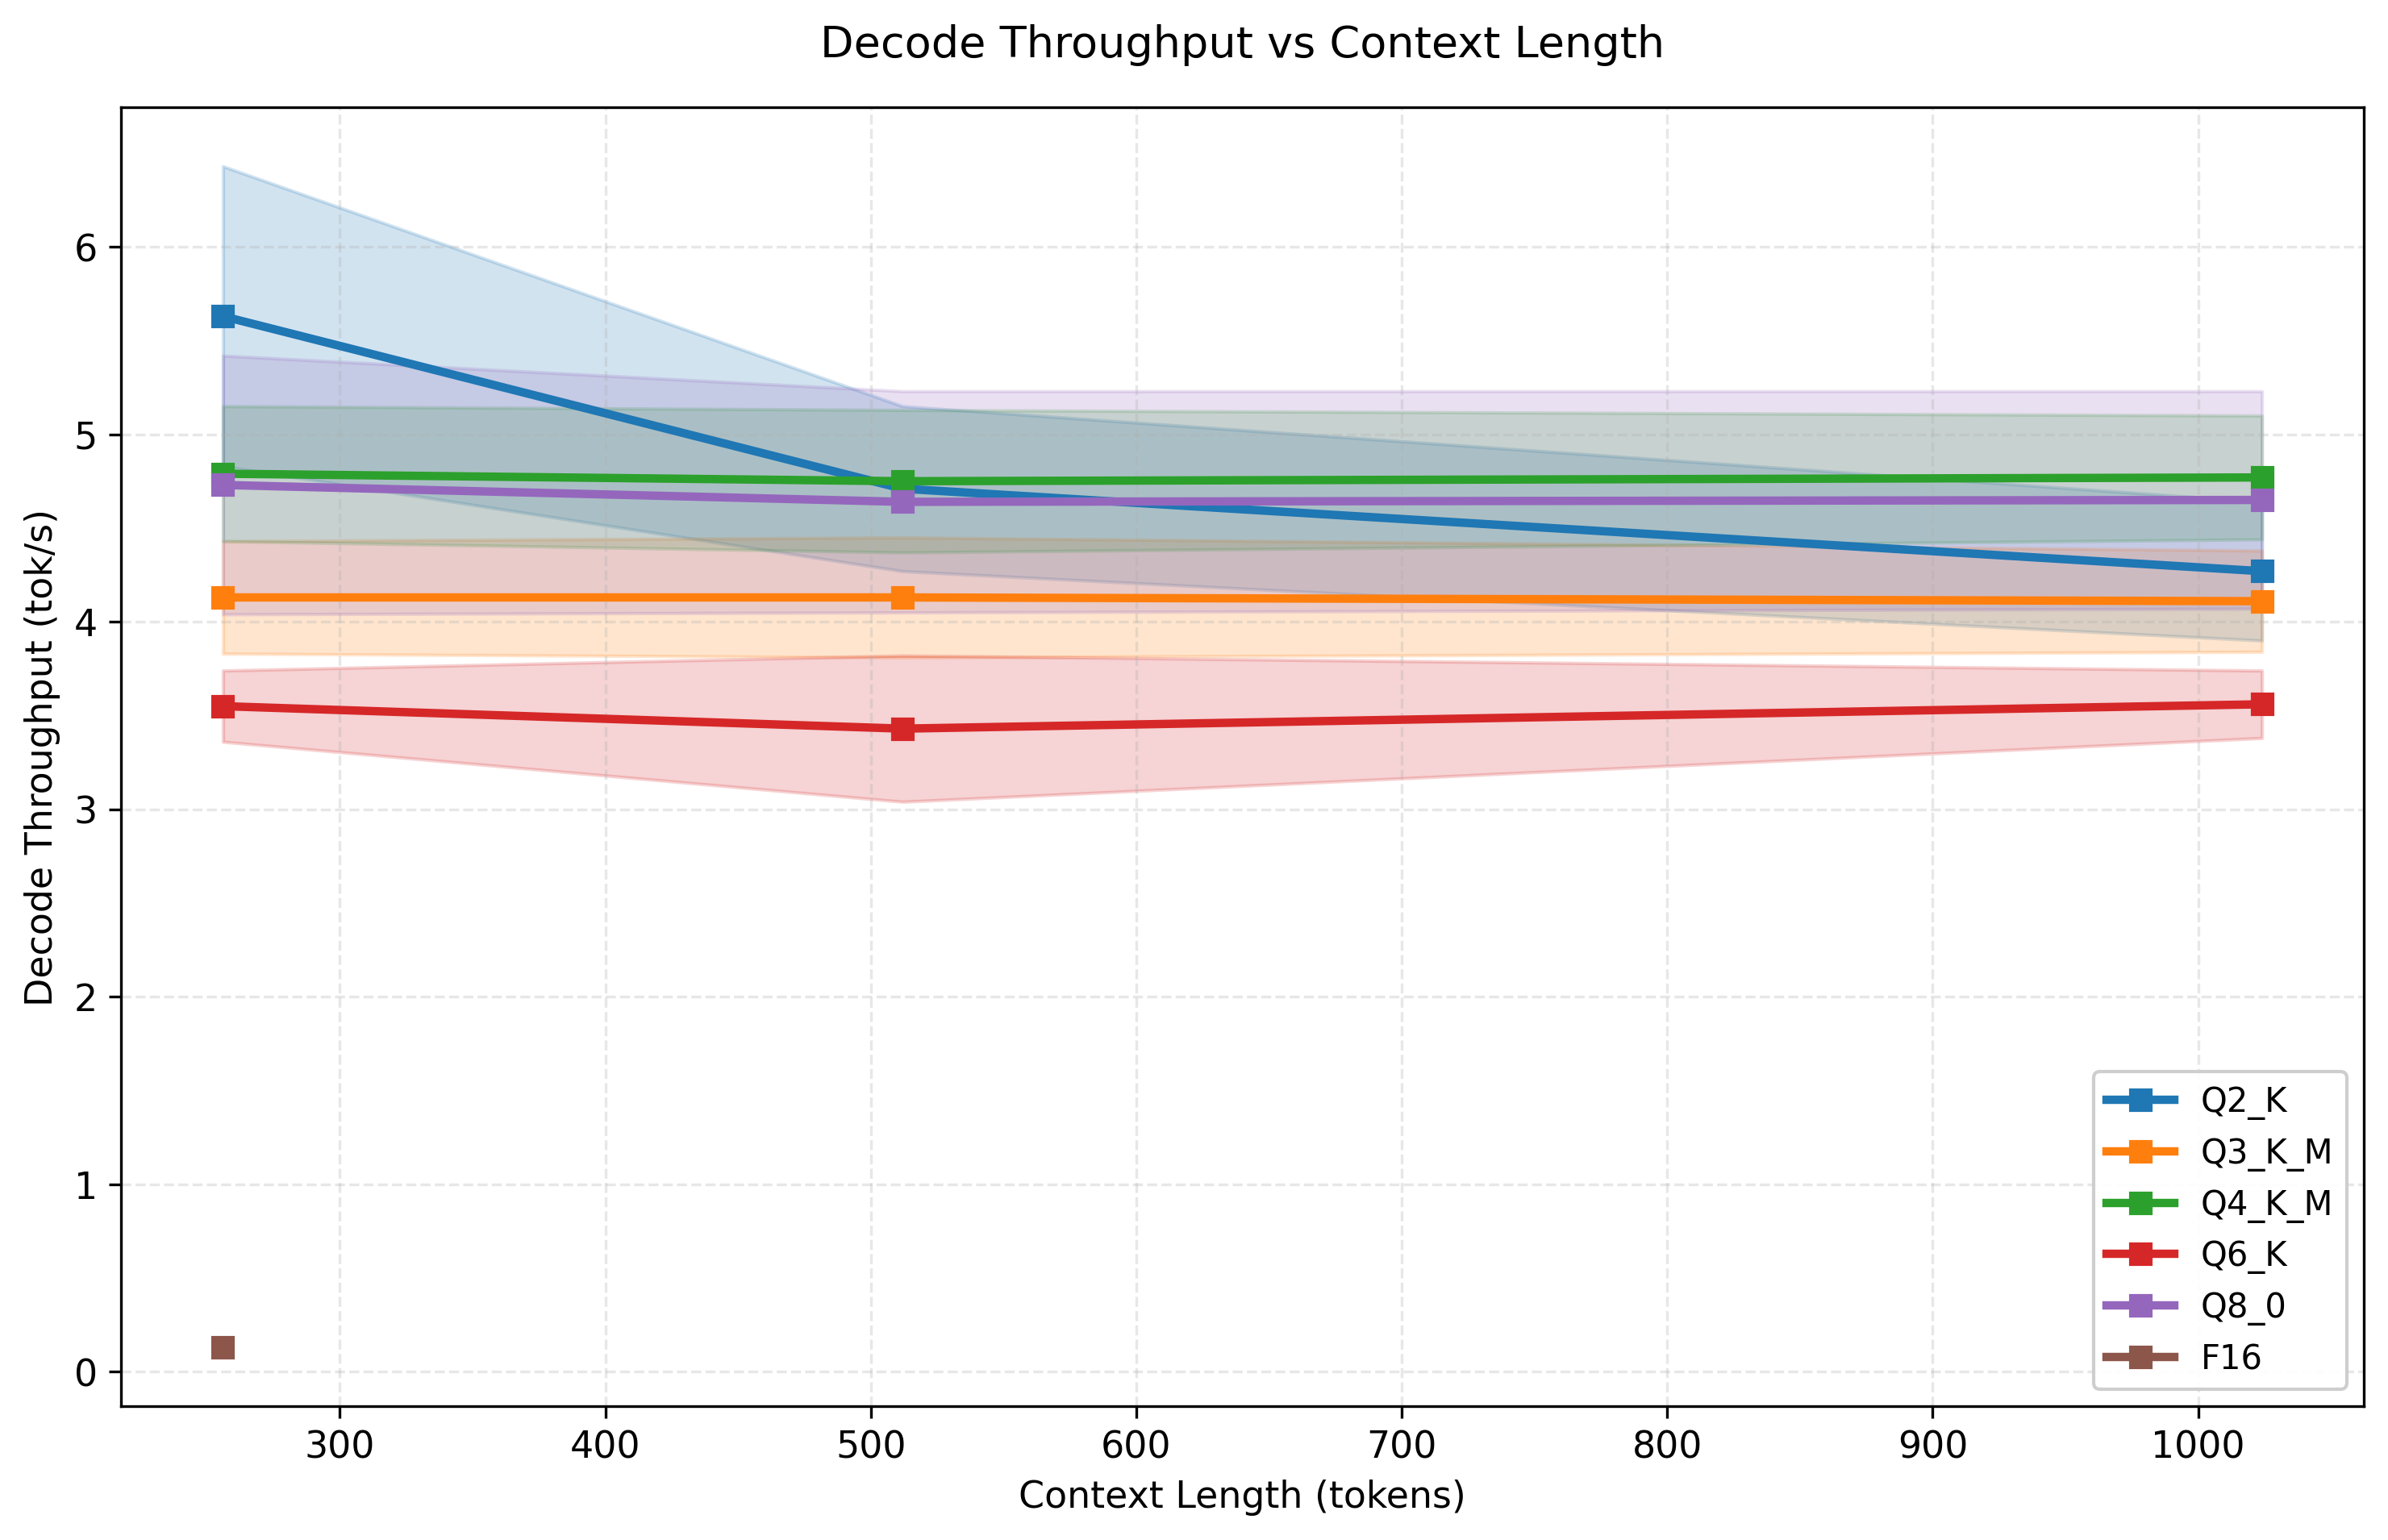
\includegraphics[width=\columnwidth]{../figures/fig2_decode_tps_vs_context.png}
  \caption{Decode throughput (tokens/s) across KV-cache context window sizes
  for all variants (error bars: $\pm 1$ std, $n{=}15$/cell). Q3\_K\_M and Q6\_K
  collapse at ctx=2048 ($-43\%$ and $-52\%$ relative to ctx=1024) while Q4\_K\_M
  ($+2\%$) and Q2\_K ($-5\%$) remain stable.}
  \label{fig:ctx_sweep}
\end{figure}

Table~\ref{tab:ctx2048} and Figure~\ref{fig:ctx_sweep} present decode throughput
across all four KV-cache window sizes for the five non-F16 variants.

\begin{table}[h]
\centering
\caption{Decode TPS (mean$\pm$std, $n{=}15$/cell) by variant and KV-cache
context window size. \textbf{Bold} = $>$10\% decline from ctx=1024.
$\Delta$ = fractional change from ctx=1024 to ctx=2048.}
\label{tab:ctx2048}
\setlength{\tabcolsep}{3pt}
\footnotesize
\begin{tabular}{@{}lrrrrc@{}}
\toprule
\textbf{Var.} & \textbf{ctx=256} & \textbf{ctx=512} & \textbf{ctx=1024} & \textbf{ctx=2048} & \textbf{$\Delta$} \\
\midrule
Q2\_K    & 5.66{\tiny$\pm$.72} & 5.05{\tiny$\pm$.48} & 4.83{\tiny$\pm$.43} & 4.60{\tiny$\pm$.48} & $-5\%$ \\
Q3\_K\_M & 4.91{\tiny$\pm$.40} & 4.82{\tiny$\pm$.35} & 4.81{\tiny$\pm$.38} & \textbf{2.76{\tiny$\pm$.87}} & $-43\%$ \\
Q4\_K\_M & 4.79{\tiny$\pm$.36} & 5.32{\tiny$\pm$.52} & 5.18{\tiny$\pm$.50} & 5.26{\tiny$\pm$.25} & $+2\%$ \\
Q6\_K    & 3.98{\tiny$\pm$.32} & 4.03{\tiny$\pm$.39} & 4.01{\tiny$\pm$.34} & \textbf{1.94{\tiny$\pm$.26}} & $-52\%$ \\
Q8\_0    & 4.95{\tiny$\pm$.59} & 4.95{\tiny$\pm$.68} & 4.83{\tiny$\pm$.70} & \textbf{4.23{\tiny$\pm$.49}} & $-12\%$ \\
\bottomrule
\end{tabular}
\end{table}

The results reveal three distinct behavioral regimes:

\textbf{Context-stable variants (Q4\_K\_M, Q2\_K).} Q4\_K\_M varies by only
$\pm$11\% across the full 256--2048 range (4.79 to 5.32 tok/s), with no
monotonic trend. Q2\_K shows a gradual 5\% decline from ctx=256 to ctx=2048
(5.66 to 4.60 tok/s), well within the noise band. Both variants are safe for
long-context deployment.

\textbf{Mildly sensitive (Q8\_0).} Q8\_0 declines 12\% from ctx=1024 to
ctx=2048 (4.83 to 4.23 tok/s), a statistically meaningful but operationally
acceptable degradation. Q8\_0 remains usable at ctx=2048 with a known
performance cost.

\textbf{Catastrophically sensitive (Q3\_K\_M, Q6\_K).} Q3\_K\_M drops
from 4.81 to 2.76 tok/s ($-43\%$) at ctx=2048. Q6\_K drops from 4.01 to
1.94 tok/s ($-52\%$)---below the interactive threshold and in the same range
as F16's non-functional 0.15 tok/s. The std for Q3\_K\_M at ctx=2048
is $\pm$0.87 tok/s, notably higher than at other context sizes, suggesting
the memory system enters an intermittent pressure regime rather than a clean
new steady state.

\subsection{KV-Cache Size Calculation}

The 2048-token KV-cache for Llama~3.2~3B occupies:
\[
  2 \times 28 \times 8 \times 128 \times 2048 \times 2~\text{bytes} \approx 234~\text{MB}
\]

For Q4\_K\_M (2.0~GB weights), this KV footprint represents $\approx$11.2\%
of per-step memory traffic, keeping decode firmly weight-bandwidth-bound.
For Q6\_K (2.7~GB weights), the fraction is $\approx$8.3\%---even smaller---yet
Q6\_K collapses at ctx=2048 while Q4\_K\_M does not. This rules out a
simple ``total bytes'' explanation.

\subsection{Mechanistic Hypothesis: NEON Kernel Memory Access Amplification}

The asymmetry between Q6\_K's collapse and Q4\_K\_M's stability, despite
Q6\_K having a smaller KV-fraction of memory traffic, points to a
\emph{kernel-level} difference. Q6\_K's dequantization kernel uses a
multi-step 4-bit$+$2-bit unpacking pipeline requiring more DRAM reads per
weight than Q4\_K\_M's streamlined 4-bit dot-product kernel. At smaller
KV-cache sizes, this overhead is hidden by the LPDDR5 controller's prefetcher,
which can amortize irregular access patterns across a manageable working set.
When the KV-cache grows to 234~MB, the prefetcher's effective coverage is
reduced, and the irregular access pattern of Q6\_K's kernel begins to incur
DRAM-latency penalties that are proportional to its higher effective access
count per inference step. Q4\_K\_M's more regular access pattern remains
prefetcher-friendly even at the larger working set.

Q3\_K\_M's collapse is less severe ($-43\%$ vs.\ $-52\%$ for Q6\_K) but
follows the same mechanism: its medium-complexity block structure with
finer-granularity scale lookups incurs higher access amplification than
Q4\_K\_M but less than Q6\_K.

\subsection{TTFT Grows with KV-Cache Window Size}

\begin{figure}[t]
  \centering
  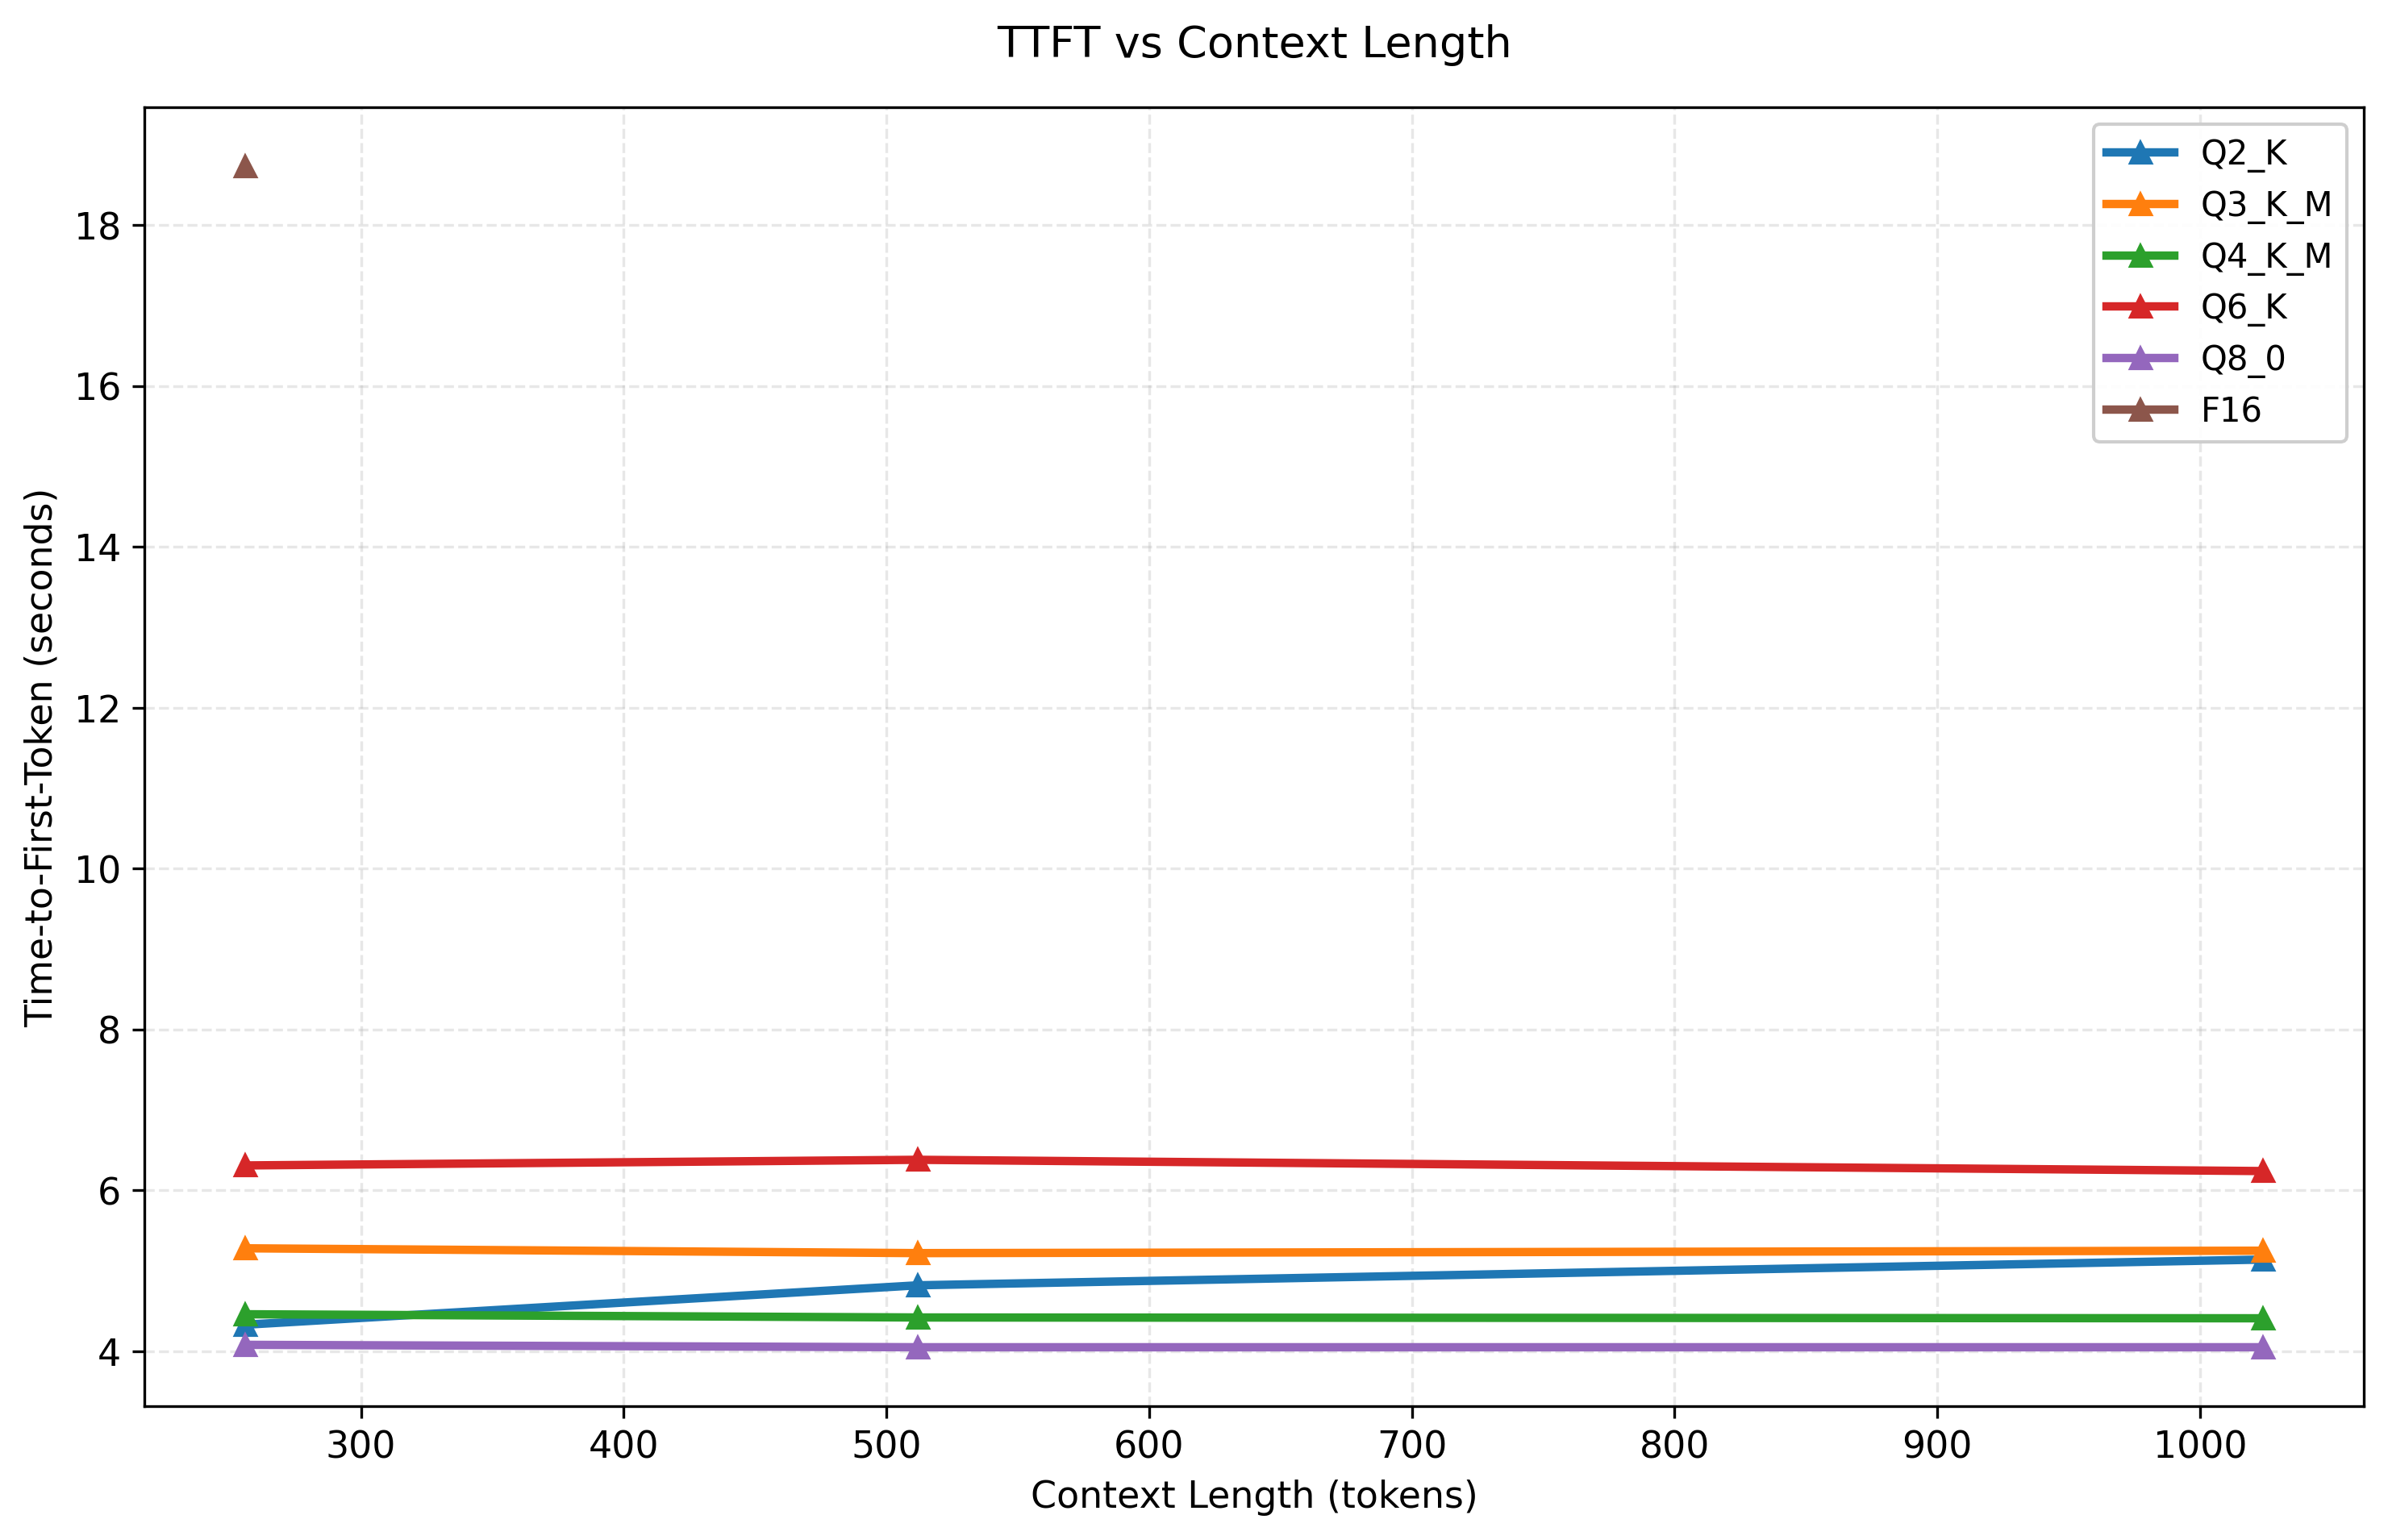
\includegraphics[width=\columnwidth]{../figures/fig3_ttft_vs_context.png}
  \caption{Time-to-first-token (seconds) as a function of KV-cache context
  window size. TTFT grows uniformly across variants due to larger KV-cache
  initialization cost, \emph{not} longer input sequences.}
  \label{fig:ttft}
\end{figure}

Figure~\ref{fig:ttft} shows that TTFT grows with KV-cache window size
uniformly across all variants. For context-stable variants like Q4\_K\_M,
TTFT growth is the \emph{only} metric that increases with the \texttt{-c}
parameter---an important distinction for applications that care primarily
about first-token latency (e.g., voice assistants). Practitioners should
budget TTFT carefully when setting KV-cache window parameters.

% ===========================================================================
\section{Results: Quality Evaluation}
\label{sec:quality}
% ===========================================================================

\subsection{BoolQ Reading Comprehension}

On-device BoolQ accuracy was measured for all six variants via USB ADB
(100 questions per variant). Results with 95\% Wilson CIs are shown in
Table~\ref{tab:main_results}. The accuracy ordering is:

\begin{align*}
  \text{Q4\_K\_M}\,(72\%) &> \text{Q2\_K}\,(69\%) > \text{Q8\_0}\,(68\%) > \text{F16}\,(68\%) \\
                          &> \text{Q3\_K\_M}\,(66\%) > \text{Q6\_K}\,(65\%)
\end{align*}

This ordering is \textbf{non-monotonic with bit-width}. The 4-bit Q4\_K\_M
achieves the highest accuracy, while the 6-bit Q6\_K scores lowest---7 percentage
points below Q4\_K\_M despite having 50\% more bits per weight. The 7-point gap
between Q4\_K\_M and Q6\_K is the most statistically robust distinction given
the $\pm$8--9\% Wilson CI: the CI intervals [63--80\%] vs.\ [55--74\%] overlap
substantially, meaning this gap alone does not reach statistical significance
at $n{=}100$. The result is directionally clear but would benefit from a larger
evaluation set.

Notably, F16 (full precision, 68\%) does not outperform Q4\_K\_M (72\%).
This counterintuitive result likely reflects sampling variance at $n{=}100$
and the well-documented finding that quantization errors in K-quant schemes
are not always accuracy-reducing on specific downstream tasks.

\subsection{ARC-Easy: Ceiling Effect}

All quantized variants (Q2\_K through Q8\_0) scored 100\% on ARC-Easy
elementary science questions. F16 scored 95\% (19/20 errors). This ceiling
effect confirms that ARC-Easy is too easy for this model class and cannot
serve as a quality discriminator among quantization variants. The result
is consistent with broader observations about Llama 3.2 3B's strong factual
recall capacity.

\textbf{Honest note on benchmark design.} The ARC-Easy ceiling effect was
anticipated after observing near-ceiling performance in a small pilot.
The 100-question subset was maintained for comparability, but ARC-Challenge
(harder questions from the same dataset) would provide better discriminative
power. This is identified as a priority for future work.

\subsection{Perplexity vs.\ Task Accuracy Divergence}

Full-corpus WikiText-2 PPL (${\approx}$285K tokens) is available for Q2\_K
(PPL = 13.29) and Q3\_K\_M (PPL = 11.08). These PPL values suggest Q3\_K\_M
has meaningfully better language model quality than Q2\_K---yet Q3\_K\_M scores
\emph{lower} on BoolQ (66\%) than Q2\_K (69\%). This divergence between
perplexity and task accuracy is a well-documented phenomenon in the quantization
literature and confirms that WikiText-2 PPL is an insufficient proxy for
reading-comprehension quality.

For Q4\_K\_M, Q6\_K, and Q8\_0, PPL was measured on a 12~KB sample only
(corpus\_bytes = 12,014 per \texttt{perplexity\_scores.json}). The sample
values (Q4\_K\_M: 9.76, Q6\_K: 9.75, Q8\_0: 9.70) are likely compressed
relative to full-corpus values---12~KB is insufficient to characterize
long-range language model quality. These values should be treated as
approximate, and direct comparison to the Q2\_K/Q3\_K\_M full-corpus PPL
is not methodologically valid.

The honest conclusion: on-device task evaluation (BoolQ, ARC) provides more
reliable deployment guidance than PPL for this model class. Full-corpus PPL
re-runs for all five variants are planned and listed in Section~\ref{sec:future}.

% ===========================================================================
\subsection{imatrix Calibration Quality}
\label{sec:imatrix}
% ===========================================================================

Importance-matrix (imatrix) calibration requantizes each GGUF variant using
per-tensor activation statistics collected over 65{,}536 WikiText-2 calibration
tokens, biasing bit allocation toward salient weights. We evaluate BoolQ
accuracy for all seven imatrix variants on the Pixel~6a.

\begin{table}[ht]
\centering
\caption{BoolQ accuracy: imatrix-calibrated variants vs.\ standard variants
(100 questions, Wilson 95\% CI). Higher is better.}
\label{tab:imatrix_boolq}
\begin{tabular}{lrr}
\toprule
\textbf{Variant} & \textbf{Accuracy} & \textbf{$\pm$CI} \\
\midrule
Q2\_K-imatrix   & 64.0\% & $\pm$9.2\% \\
Q3\_K\_M-imatrix & 61.0\% & $\pm$9.4\% \\
Q4\_K\_S-imatrix & 75.0\% & $\pm$8.4\% \\
Q4\_K\_M-imatrix & 71.0\% & $\pm$8.8\% \\
Q5\_K\_M-imatrix & 68.0\% & $\pm$9.0\% \\
Q6\_K-imatrix   & 69.0\% & $\pm$8.9\% \\
Q8\_0-imatrix   & 68.0\% & $\pm$9.0\% \\
\bottomrule
\end{tabular}
\end{table}

Three findings stand out. First, Q4\_K\_S-imatrix achieves the highest BoolQ
accuracy (75.0\%) of all seven imatrix variants---surpassing even Q4\_K\_M-imatrix
(71.0\%) and Q8\_0-imatrix (68.0\%). This is a non-trivial result: a smaller
superblock granularity combined with importance-weighted calibration outperforms
larger bit-widths on this task, suggesting that calibration quality interacts
with quantization structure in ways not captured by bits-per-weight alone.

Second, very low-bit variants (Q2\_K-imatrix, Q3\_K\_M-imatrix) lag at
64\% and 61\% respectively, indicating that imatrix calibration cannot fully
recover task quality at 2--3 bits. The calibration redistributes bits toward
important weights, but the total information capacity at these widths remains
a hard constraint.

Third, Q5\_K\_M-imatrix, Q6\_K-imatrix, and Q8\_0-imatrix converge to similar
accuracy (68--69\%), consistent with diminishing returns above $\approx$5 bits
and suggesting Q5\_K\_M-imatrix as the practical Pareto frontier for
accuracy-efficiency trade-off with imatrix calibration.

% ===========================================================================
\section{Discussion}
\label{sec:discussion}
% ===========================================================================

\subsection{Why Q6\_K is Pareto-Dominated}

Q6\_K is simultaneously the slowest practical variant (3.98 tok/s at ctx=256,
1.94 tok/s at ctx=2048) and the least accurate on BoolQ (65\%).
There is no deployment scenario on CPU-only mobile hardware in which Q6\_K
is the correct choice:
\begin{itemize}
  \item If throughput matters: Q4\_K\_M (5.32 tok/s) and Q2\_K (5.66 tok/s)
        are both faster.
  \item If accuracy matters: Q4\_K\_M (72\%) is more accurate.
  \item If memory matters: Q4\_K\_M (2.0~GB) is smaller.
  \item If long context is needed: Q4\_K\_M is stable at ctx=2048 ($+2\%$);
        Q6\_K collapses to 1.94 tok/s ($-52\%$).
\end{itemize}

The intuition that Q6\_K should provide ``near-lossless'' quality at modest
size overhead is correct in principle but does not materialize on this
hardware-kernel combination. The Q6\_K de-quantization kernel for ARM NEON
imposes overhead that offsets its bit-width advantage in all measured
dimensions.

\subsection{Deployment Decision Framework}

Based on the experimental results, we propose the following deployment
decision tree for practitioners targeting ARM mobile hardware with llama.cpp:

\begin{itemize}
  \item \textbf{Default (any 4+ GB device)}: Q4\_K\_M. Best overall balance:
        72\% BoolQ, 5.32 tok/s, 2.0~GB, context-stable, low variance (std 0.52).
  \item \textbf{RAM-constrained (3~GB device) or latency-critical}: Q2\_K.
        Fastest at 5.66 tok/s, smallest at 1.3~GB, 69\% BoolQ.
  \item \textbf{Quality-maximizing (6+ GB device, ctx $\leq$ 1024)}: Q8\_0.
        Mild 12\% ctx-2048 degradation; useful when quality above Q4\_K\_M
        is needed and context will stay below 1024 tokens.
  \item \textbf{Avoid}: Q6\_K (dominated on all axes on CPU backends).
        Q3\_K\_M (unstable at ctx=2048; lower accuracy than Q2\_K despite
        larger size).
  \item \textbf{Thread count}: Always use 4 threads on 4-performance-core
        ARM big.LITTLE SoCs; do not enable little-core threads.
  \item \textbf{KV-cache planning}: Budget TTFT growth with window size. Use
        Q4\_K\_M or Q2\_K for ctx $\geq$ 2048; hard-limit Q3\_K\_M and Q6\_K
        to ctx $\leq$ 1024.
\end{itemize}

\subsection{Comparison to Desktop CPU Findings}

The arXiv:2601.14277 study~\cite{whichquant} finds Q5\_K\_M to be the optimal
GGUF variant on Apple M2 (Llama 3.1 8B). Our study finds Q4\_K\_M optimal on
the Tensor G1 (Llama 3.2 3B). The difference is informative.

Apple M2 has unified memory architecture with higher and more consistent
bandwidth (100+ GB/s theoretical), and Apple's own Metal-accelerated NEON
kernels are more uniformly optimized across variants. The higher bandwidth
reduces the relative cost of the Q6\_K dequantization overhead and shifts
the optimal point one step higher in bit-width. On the Tensor G1, the
lower and less consistent LPDDR5 bandwidth (25--35~GB/s application-layer)
amplifies kernel overhead differences, shifting the optimum downward to
Q4\_K\_M.

This comparison suggests that the Q4\_K\_M optimum may be specific to
Android LPDDR5 platforms, and that Snapdragon and MediaTek devices with
higher memory bandwidth might find a different optimal point.

\subsection{Limitations}

This study has several important limitations that bound the generalizability
of its findings:

\textbf{Single device.} All 661 measurements are from a single Google Pixel 6a.
The Tensor G1's specific LPDDR5 bandwidth, memory controller behavior, and
NEON kernel optimization profile may not generalize to Snapdragon 8 Gen 3,
MediaTek Dimensity, or Apple A-series SoCs. The KV-cache collapse effect in
particular is tied to the specific memory subsystem behavior of this device.

\textbf{Single model family.} All results use Llama 3.2 3B Instruct.
Different model architectures (different numbers of KV heads, layer counts,
or attention mechanisms) would produce different absolute KV-cache sizes and
potentially different sensitivity profiles.

\textbf{No NPU baseline.} The Tensor G1 includes an Arm Mali-G78 GPU and a
Google TPU block. This study uses CPU-only inference (llama.cpp NDK backend).
NPU-accelerated backends might produce a completely different variant ordering.

\textbf{Limited F16 data.} Only 2 successful F16 trials were completed. All
F16 statistics are from this minimal sample and should be treated as
illustrative only.

\textbf{PPL measurement gap.} Three of five variants have PPL measured on a
12~KB sample rather than the full test corpus, making cross-variant PPL
comparisons unreliable.

\textbf{No energy measurement.} The WiFi ADB protocol records battery
percentage changes, but Android's integer-only battery reporting is too
coarse for per-trial energy accounting. A hardware power monitor would be
required for reliable per-variant energy characterization.

% ===========================================================================
\section{Future Work}
\label{sec:future}
% ===========================================================================

The present study establishes a baseline and identifies several high-priority
follow-up experiments. In roughly priority order:

\textbf{(1) Granular ctx collapse sweep.}
The Q3\_K\_M and Q6\_K collapses are observed at ctx=2048 but not ctx=1024.
A granular sweep at 1024, 1280, 1536, 1792, and 2048 tokens would identify
the collapse threshold, which is critical deployment information.

\textbf{(2) KV-cache quantization mitigation.}
llama.cpp supports Q8\_0 quantization of the KV cache
(\texttt{-ctk q8\_0 -ctv q8\_0}), halving the 234~MB KV footprint at ctx=2048
to ${\approx}$117~MB. Testing whether this flag mitigates the Q3\_K\_M and
Q6\_K collapses without accuracy regression is an immediately tractable
experiment requiring no new model quantizations.

\textbf{(3) Importance-matrix (imatrix) calibration.}
Re-quantizing the model using an importance-weighted calibration corpus
(\texttt{llama-imatrix}) may improve BoolQ accuracy at Q2\_K and Q3\_K\_M
by better preserving high-salience weights. The comparison baseline (standard
vs.\ imatrix-calibrated) is a controlled experiment with the same binary and
hardware.

\textbf{(4) Additional quality benchmarks.}
ARC-Challenge (harder), HellaSwag (commonsense), MMLU (knowledge breadth),
and TruthfulQA (factual accuracy) would provide a richer quality profile and
better discriminate between the middle-range variants (Q2\_K, Q8\_0,
Q3\_K\_M). The non-monotonic BoolQ ordering warrants confirmation across
multiple benchmarks.

\textbf{(5) Full-corpus PPL re-run.}
Re-evaluating Q4\_K\_M, Q6\_K, and Q8\_0 PPL on the full 285K-token
WikiText-2 test corpus would validate the partial PPL values and enable
reliable cross-variant perplexity comparisons.

\textbf{(6) Cross-device benchmarking.}
Repeating this study on Snapdragon 8 Gen 3 (Qualcomm), Apple M4 (Mac mini),
and Intel x86 with AVX2 would establish whether the non-monotonic throughput
finding and KV-cache collapse effects generalize across ARM SoC families and
non-ARM architectures. The current PROJECT\_PLAN targets a 4-device study
(Pixel 6a, Mac M4, iPhone 14 Pro A16, HP Pavilion x86 AVX2).

\textbf{(7) Cross-model validation.}
Spot-checking Q4\_K\_M throughput on Qwen2.5-1B and Gemma~3~1B at the same
hardware configuration would verify that the findings are not specific to
Llama's architectural choices (grouped query attention, RoPE configuration).

% ===========================================================================
\section{Conclusion}
% ===========================================================================

We have presented a rigorous systems benchmarking study of six GGUF quantization
variants of Llama~3.2~3B Instruct on a Google Pixel~6a (Tensor G1, 6~GB LPDDR5),
yielding 661 valid measurements across four KV-cache window sizes (256--2048 tokens),
five quantization levels, and a thread-count scaling study.

Our four key findings are:

\begin{enumerate}
  \item \textbf{Non-monotonic throughput.} Q6\_K (6-bit, 2.7~GB) delivers only
        3.98~tok/s---slower than Q4\_K\_M (5.32~tok/s) and Q8\_0 (4.95~tok/s)---due
        to dequantization kernel overhead on ARM NEON. The throughput ordering
        is Q2\_K $>$ Q4\_K\_M $>$ Q8\_0 $\approx$ Q3\_K\_M $\gg$ Q6\_K, not
        the bandwidth-only prediction.

  \item \textbf{Variant-specific KV-cache sensitivity.} Q4\_K\_M ($+2\%$) and
        Q2\_K ($-5\%$) are stable through ctx=2048; Q8\_0 shows mild $-12\%$
        decline. Q3\_K\_M and Q6\_K collapse catastrophically at ctx=2048
        ($-43\%$ and $-52\%$ respectively), making them unsafe for
        maximum-context deployments. This is the first characterization of
        this effect on Android ARM hardware.

  \item \textbf{Non-monotonic accuracy.} On BoolQ reading comprehension,
        Q4\_K\_M achieves the highest accuracy (72\%) while Q6\_K scores
        lowest (65\%), despite its higher bit-width. ARC-Easy is near-ceiling
        for all variants and is not a useful quality discriminator.

  \item \textbf{Q6\_K is strictly dominated.} Q6\_K offers no advantage over
        Q4\_K\_M or Q8\_0 on any measured dimension---throughput, accuracy,
        model size, or context stability---on CPU-only ARM backends.
\end{enumerate}

The practical deployment recommendation is: use Q4\_K\_M as the default for
6~GB Android devices (highest BoolQ accuracy, context-stable, best overall
balance); use Q2\_K when latency or RAM is the primary constraint; use 4 threads
on big.LITTLE ARM (not all cores); and avoid Q6\_K entirely on CPU inference
backends.

As on-device AI continues to proliferate across consumer hardware, hardware-specific
empirical benchmarks of this kind are essential for evidence-based quantization
selection. Specifications alone do not predict deployment behavior on mobile
ARM SoCs.

% ===========================================================================
\begin{thebibliography}{99}

\bibitem{llama32}
Meta AI, ``Llama 3.2: Lightweight and Vision Language Models,''
Meta AI Blog, September 2024. [Online]. Available:
\url{https://ai.meta.com/blog/llama-3-2-connect-2024-vision-edge-mobile-devices/}

\bibitem{llamacpp}
G. Gerganov et al., ``llama.cpp: Efficient LLM inference in C/C++,''
GitHub Repository, 2023--2025. [Online]. Available:
\url{https://github.com/ggerganov/llama.cpp}

\bibitem{gguf}
G. Gerganov, ``GGUF: A File Format for Language Model Weights,''
GitHub, llama.cpp project, 2023. [Online]. Available:
\url{https://github.com/ggerganov/ggml/blob/master/docs/gguf.md}

\bibitem{whichquant}
C. Xu, F. Tang, Y. Ma, B. Xu, Z. Xu, C. Zhu, X. Wang, and T. Lu,
``Which Quantization is Right for Me? Comparing Inference Efficiency of Quantized Large
Language Models on Consumer Hardware,''
arXiv preprint arXiv:2601.14277, 2026.

\bibitem{mobileaibench}
W. Murugadoss, S. Xu, S. Chandra, S. Movva, A. Park, P. Chen, B. T. Lau,
Y. Li, and A. Philipose,
``MobileAIBench: Benchmarking LLMs and LMMs for On-Device Use Cases,''
arXiv preprint arXiv:2406.10290, 2024.

\bibitem{armkernels}
K. Balasubramanian et al.,
``Highly Optimized Kernels for LLM Inference on ARM CPUs,''
arXiv preprint arXiv:2501.00032, 2025.

\bibitem{kvswap}
S. Lim et al.,
``KVSwap: Bandwidth-Optimized KV Cache Swapping for Mobile LLM Inference,''
arXiv preprint arXiv:2511.11907, 2025.

\bibitem{boolq}
C. Clark, K. Lee, M.-W. Chang, T. Kwiatkowski, M. Collins, and K. Toutanova,
``BoolQ: Exploring the Surprising Difficulty of Natural Yes/No Questions,''
in \textit{Proc. NAACL-HLT}, 2019.

\bibitem{arc}
P. Clark, I. Cowhey, O. Etzioni, T. Khot, A. Sabharwal, C. Schoenick, and O. Tafjord,
``Think you have Solved Question Answering? Try ARC, the AI2 Reasoning Challenge,''
arXiv preprint arXiv:1803.05457, 2018.

\bibitem{gptq}
E. Frantar, S. Ashkboos, T. Hoefler, and D. Alistarh,
``GPTQ: Accurate Post-Training Quantization for Generative Pre-trained Transformers,''
in \textit{Proc. ICLR}, 2023.

\bibitem{awq}
J. Lin, J. Tang, H. Tang, S. Yang, X. Dang, and S. Han,
``AWQ: Activation-aware Weight Quantization for LLM Compression and Acceleration,''
in \textit{Proc. MLSys}, 2024.

\bibitem{mlcllm}
T. Chen et al., ``MLC-LLM: Universal LLM Deployment Engine with ML Compilation,''
arXiv preprint arXiv:2404.01373, 2024.

\bibitem{executorch}
Meta AI, ``ExecuTorch: On-Device AI across Mobile, Embedded, and Edge for PyTorch,''
GitHub Repository, 2024. [Online]. Available:
\url{https://github.com/pytorch/executorch}

\bibitem{androidndk}
Google, ``Android NDK: Native development for Android,''
Android Developers, 2024. [Online]. Available:
\url{https://developer.android.com/ndk}

\bibitem{tang_eval}
Y. Tang et al.,
``Evaluating Quantized Large Language Models,''
arXiv preprint arXiv:2402.18158, 2024.

\bibitem{leviathan_speculative}
Y. Leviathan, M. Kalman, and Y. Matias,
``Fast Inference from Transformers via Speculative Decoding,''
in \textit{Proc. ICML}, 2023. arXiv:2211.17192.

\bibitem{kvquant}
C. Hooper et al.,
``KVQuant: Towards 10 Million Context Length LLM Inference with KV Cache Quantization,''
arXiv preprint arXiv:2401.18079, 2024.

\bibitem{smoothquant}
G. Xiao, J. Lin, M. Seznec, H. Wu, J. Demouth, and S. Han,
``SmoothQuant: Accurate and Efficient Post-Training Quantization for Large Language Models,''
in \textit{Proc. ICML}, 2023.

\end{thebibliography}

% ===========================================================================
\appendix
% ===========================================================================

\section{Experimental Reproducibility}

\subsection{Build Configuration}

The llama.cpp library was compiled from commit \texttt{b1-1a29907} using
Android NDK version 29.0.14206865. Key compilation flags:
\begin{verbatim}
-O3 -march=armv8.2-a+dotprod+fp16
-DGGML_USE_CPU_HBM=OFF
-DLLAMA_BUILD_TESTS=OFF
\end{verbatim}

The \texttt{llama-cli} binary was pushed to \texttt{/data/local/tmp/} on
the device. The Android app was compiled with NDK 29.0.14206865, targeting
arm64-v8a, using CMake 4.2.3 and Gradle 8.x.

\subsection{Invocation Template}

\begin{verbatim}
./llama-cli \
  -m <model_path>.gguf \
  -p "<system_prompt><user_prompt>" \
  -n 128 \
  --ctx-size <context_length> \
  --seed <trial_seed> \
  -t <thread_count> \
  --log-format json
\end{verbatim}

\subsection{Statistical Methodology}

Means and standard deviations in Table~\ref{tab:main_results} are computed
across 15 samples per variant per context (5 trials $\times$ 3 prompt types).
Warmup runs (2 per configuration) are excluded. Outlier rejection was not
applied; all completed trials within the timeout threshold are included.

\section{Quality Evaluation Details}

\subsection{BoolQ Prompt Template}

\begin{verbatim}
Passage: {passage}
Question: {question}
Answer with only yes or no:
\end{verbatim}

Responses are scored by extracting the first occurrence of ``yes'' or ``no''
(case-insensitive) from the model output within 400 characters following
the instruction marker.

\subsection{ARC-Easy Prompt Template}

\begin{verbatim}
Question: {question}
Choices: A) {A} B) {B} C) {C} D) {D}
Answer with only A, B, C, or D:
\end{verbatim}

Scoring uses exact-match on the predicted letter (A/B/C/D) against the
ground truth from the AI2 ARC Easy test split.

\subsection{Perplexity Evaluation}

WikiText-2 perplexity was evaluated using the \texttt{llama-perplexity}
command from the same llama.cpp build. Q2\_K and Q3\_K\_M were evaluated
on the full test corpus (${\approx}$285K tokens). Q4\_K\_M, Q6\_K, and Q8\_0
were evaluated on a 12,014-byte sample due to time constraints; these values
are not directly comparable to the full-corpus Q2\_K/Q3\_K\_M results and
are marked $\ddagger$ throughout.

\end{document}
